\documentclass[review]{elsarticle}

\usepackage{lineno,hyperref}
\usepackage{amssymb,amsmath}
\usepackage{algorithm,algpseudocode}
%\usepackage[margin=2.5cm]{geometry}
\modulolinenumbers[5]

\journal{Information Processing Letters}
\bibliographystyle{elsarticle-num}

\newtheorem{theorem}{Theorem}
\newtheorem{lemma}[theorem]{Lemma}

\def\QED{\ensuremath{{\square}}}
\def\markatright#1{\leavevmode\unskip\nobreak\quad\hspace*{\fill}{#1}}
\newenvironment{proof}
{\begin{trivlist}\item[\hskip\labelsep{\bf Proof.}]}
  {\markatright{\QED}\end{trivlist}}

%%%%%%%%%%%%%%%%%%%%%%%
%% Elsevier bibliography styles
%%%%%%%%%%%%%%%%%%%%%%%
%% To change the style, put a % in front of the second line of the current style and
%% remove the % from the second line of the style you would like to use.
%%%%%%%%%%%%%%%%%%%%%%%

%% Numbered
%\bibliographystyle{model1-num-names}

%% Numbered without titles
%\bibliographystyle{model1a-num-names}

%% Harvard
%\bibliographystyle{model2-names.bst}\biboptions{authoryear}

%% Vancouver numbered
%\usepackage{numcompress}\bibliographystyle{model3-num-names}

%% Vancouver name/year
%\usepackage{numcompress}\bibliographystyle{model4-names}\biboptions{authoryear}

%% APA style
%\bibliographystyle{model5-names}\biboptions{authoryear}

%% AMA style
%\usepackage{numcompress}\bibliographystyle{model6-num-names}

%% `Elsevier LaTeX' style
%%%%%%%%%%%%%%%%%%%%%%%

\begin{document}

\begin{frontmatter}

\title{An O(1)-Approximation Algorithm for the 2-Dimensional Geometric Freeze-Tag Problem}

%% Group authors per affiliation:
%% or include affiliations in footnotes:
\author[aut]{Ehsan Najafi Yazdi\corref{correspondingauthor}}
\cortext[correspondingauthor]{Corresponding author}
\ead{ehsan@aut.ac.ir}
\author[aut,iau]{Alireza Bagheri}
\ead{ar\_bagheri@aut.ac.ir}
\author[aut]{Zahra Moezkarimi}
\ead{zmoezkarimi@aut.ac.ir}
\author[tmu]{Hamidreza Keshavarz}
\ead{Keshavarz.h@modares.ac.ir}

\address[aut]{Computer Engineering and Information Technology Department, Amirkabir University of Technology, Tehran, Iran}
\address[iau]{Computer Engineering Department, Tehran North Branch, Islamic Azad University, Tehran, Iran}
\address[tmu]{Faculty of Electrical and Computer Engineering, Tarbiat Modares University, Tehran, Iran}

\begin{abstract}
The problem of awaking a swarm of \textit{asleep} robots, starting with only one \textit{awake} robot, is named the \textit{Freeze-Tag Problem (FTP)}. Waking up a robot is done by having an awake robot move to its position. Once a robot is awakened, it can assist in awaking others. In the FTP, the objective is to wake up all the robots in the shortest time possible. This problem is NP-Hard in general, and its geometric variant is an open problem. Arkin et al. have introduced a constant factor approximation algorithm for the \textit{geometric FTP}, which runs in $O(n\log n)$ time. In this paper, we propose a constant factor approximation algorithm for the 2-dimensional geometric FTP, which runs in linear time.
\end{abstract}

\begin{keyword}
Freeze-Tag Problem \sep Broadcasting \sep Swarm robotics \sep Approximation algorithms
\end{keyword}

\end{frontmatter}

\linenumbers

\section{Introduction}
The \textit{Freeze-Tag Problem}, abbreviated as FTP, is an optimization problem arising in swarm robotics. The objective is to awaken a swarm of robots in the shortest time possible. In the beginning, there is only one \textit{awake} robot, and the rest are asleep. Waking up a robot is done by touching it by an awake robot, i.e., an awake robot should move to the asleep robot's position. Once a robot is awakened, it can assist in awakening others. The waking up process ends when the last robot is woken up~\cite{Arkin2006}. The required time to wake up all the robots is called ``\textit{makespan}''.\\
In general, an instance of the FTP can be seen as a weighted graph, in which the nodes represent robots, and distances between nodes are shown as the weights of the edges connecting them. In this way, the awaking schedule can be represented by a directed graph. The nodes represent robots, and each directed edge shows the movement-direction of a robot to wake up another. Since each robot is awakened exactly once, and an awake robot can only wake up one robot each time, each solution is a binary spanning tree, called ``\textit{wake-up tree}''. Needless to say that the root of this tree, represents the initially awake robot, and should have only one outgoing edge. The time required to wake up all the robots (makespan) is related to the depth of the tree, that is, the length of the longest path from the root to its leaves. In other words, the problem can be seen as finding a minimum-depth binary spanning tree, whose root is given and is forced to be degree-one. Arkin et al.~\cite{Arkin2006} have proved that this is an NP-Hard problem.\\
An example of the FTP is represented in Figure~\ref{fig:example}-a, in which ``A'' is the first awake robot. An awaking schedule is shown by the arrows, which yields a makespan of 18. Figure~\ref{fig:example}-b represents the wake-up tree.
\begin{figure}[h]
  \vspace{-10pt}
  \centering
  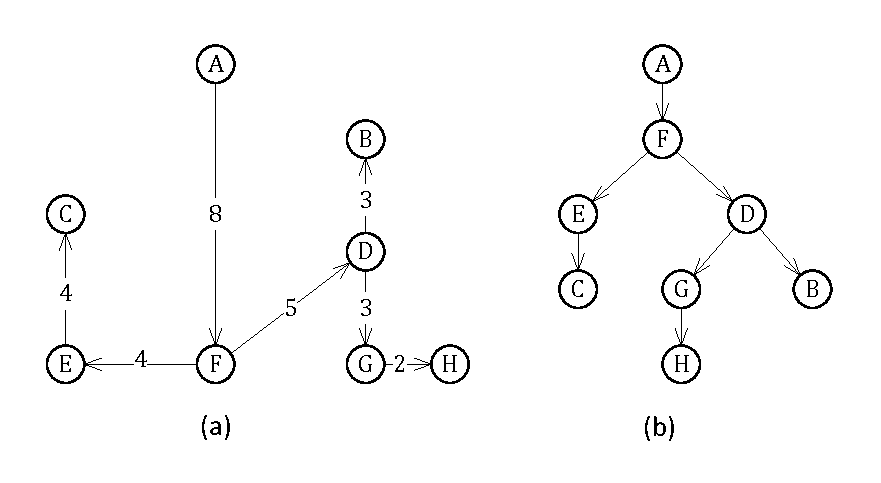
\includegraphics[scale=.7]{Figs/fig1.pdf}
  \vspace{-20pt}
  \caption{An example of the FTP (a), and its wake-up tree (b)}
  \label{fig:example}
\end{figure}

\subsection{The Geometric Freeze-Tag Problem}
One of the variants of the FTP is the geometric FTP, in which the robots are in a geometric space, and the distance between robots is the length of the line-segment connecting them. The geometric FTP is considered an open problem, and is listed as Problem \#35 on ``The Open Problems Project'' list~\cite{OpenProblems}. However there are some approximation algorithms proposed to solve it.\\
In this paper, we consider the 2-dimensional geometric FTP, and propose a constant factor approximation algorithm for solving it. The proposed algorithm improves the previous results given by Arkin et al.~\cite{Arkin2006}.

\subsection{Applications}
Besides swarm robotics, one of the main applications of the FTP is in distribution and transfer of data, and is considered when the sender and the receiver of the data should be physically near each other for transmittal. This proximity may be due to the security issues, or because of the cost of the bandwidth in wireless communications. It can be used for distributing any other duplicatable commodities, as well.
It is closely related to the \textit{Minimum maximum movement to perfect matchability (MatchMax) problem} that arises in the context of broadcasting or multicasting~\cite{Demaine2009}.\\
The FTP can also be considered as a hybrid of some problems from the areas of broadcasting, routing, scheduling, and network design~\cite{Arkin2006}. For example, it is an instance of the \textit{Cooperative Travelling Salesman problem (cTSP)} \cite{Armon2010}.

\subsection{Related Work}
As mentioned before, Arkin, Bender, Fekete, Mitchell, and Skutella~\cite{Arkin2006} have proved that in general, the FTP is an NP-Hard problem. In another work, Arkin, Bender, Ge, He, and Mitchell~\cite{Arkin2003} showed that even the FTP in unweighted graphs, is NP-hard. They gave an $O(1)-$approximation algorithm for the FTP in unweighted graphs.\\
Sztainberg, Arkin, Bender, and Mitchell~\cite{sztainberg2004} have studied heuristics for the FTP. They showed that the greedy strategy gives a $\Theta({\log n~}^{1-1/d})$ approximation bound, for the case that robots are in a D-dimensional space. More recently, Bucantanschi, Hoffmann, Hutson, and Kretchmar~\cite{Bucantanschi2007} proposed another heuristic called ``Neighborhood Search Technique'' for the FTP.\\
Könemann, Levin, and Sinha~\cite{Konemann2004} have studied the \textit{degree-bounded minimum diameter spanning tree} problem, which can be seen as a generalization of the FTP. They have introduced an algorithm with an $O(\sqrt{\log n})$ approximation factor for the problem.\\
%Hammar, Nilsson, and Persson~\cite{Hammar2006} have considered the online version of the FTP, where the exact locations of robots (and total number of them) are not known in advance.\\
In subsequent work on the FTP, Arkin et al.~\cite{Arkin2006} introduced a  $(1+\epsilon)-$approximation algorithm (PTAS) for the geometric FTP, which runs in $O(2^{poly(1/\epsilon)}+n\log n)$ time. They also gave an $O(1)-$approximation algorithm which runs in $O(n\log n)$ time.\\
The latter algorithm is discussed in the next section. In section 3, we introduce an $O(1)-$approximation algorithm for the 2-dimensional geometric FTP, with linear running time. The concluding remarks are given in section 4.

\section{Arkin et al.'s $O(1)-$Approximation Algorithm for the Geometric FTP}
In this section, an approximation algorithm proposed by Arkin et al.~\cite{Arkin2006} for the geometric FTP, is discussed. Its approximation factor is $O(1)$, and its time complexity is $O(n\log n)$. This algorithm generates a wake-up tree whose makespan is $O(radius(R))$, where $R$ is the point-set of positions of robots, and $radius(R)$ is the radius of this set with respect to the first awake robot, i.e., the maximum distance of the first awake robot to any other member of $R$.\\
It is assumed that the robots are located in a $D-$dimensional space, and the speeds of all robots are constant and equal to one unit of speed, so that, a robot requires $l$ units of time to travel $l$ units of distance.

\subsection{Describing the Algorithm}
For each point $v\in R$, the plane is partitioned into $K$ sectors by rays emanating from $v$ at angles of
$0, ~2\pi/K, ~2(2\pi/K), ..., ~(K-1)(2\pi/K)$ radians.
Let $u_j(v)$ denote the point (if any) of $R$ in the $j$th sector that is closest to $v$.
All the $u_j(v)$ points can be found for every $v\in R$, in $O(Kn\log n)$ time, with methods based on the standard Voronoi diagrams~\cite{Clarkson1987}.\\
Then, for each $v\in R$, the points $u_j(v)$ are sorted by their distance from $v$. Assuming that for $v$, these points are ${ u_1,~u_2,...,~u_K }$ in ascending order, the awaking strategy is as follows: when the $v$ robot wakes up, it travels the path ${ <v,~u_1,~u_2,...,~u_K> }$, and awakes the nearest robot in each non-empty sector surrounding it (Figure~\ref{fig:thetagraph}). If a robot has been woken up before $v$ reaches it, $v$ skips awaking it.
\begin{figure} [h]
  \vspace{-10pt}
  \centering
  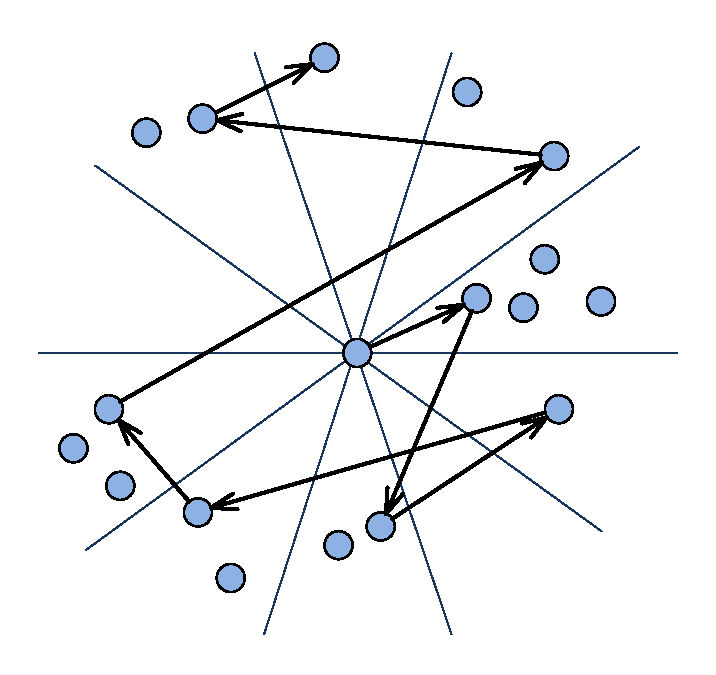
\includegraphics[scale=.5]{Figs/fig2.pdf}
  \vspace{-20pt}
  \caption{When $v$ wakes up, it awakes each of the nearest robots in the $K$ sectors surrounding it, in order of increasing distance from $v$.}
  \label{fig:thetagraph}
\end{figure}

\subsection{The Performance of the Algorithm}
Here, we discuss the performance of Arkin et al.'s algorithm. Assume that $G_K=(R,E_K)$ is a graph that connects each $v$ point to the $u_j(v)$ points that are the nearest neighbors in the $K$ sectors surrounding it. Hence, $G_K$ is a ``$\theta$-graph'' for $\theta=2\pi/K$, and if $K\geq9$, it is a ``$t_\theta-$spanner'' for ${ t_\theta=1/(\cos\theta-\sin\theta) }$~\cite{Keil1992}.
This means that the graph distance of any two nodes of the graph $G_K$ for $K\geq9$, is not greater than ${ 1/(\cos\frac{2\pi}{K}-\sin\frac{2\pi}{K}) }$ times of the Euclidean distance of those two nodes. \\
Assume the first robot is in the point $v_0$ and the last robot that is woken up by this algorithm is in the point $v_l$. How much time is required to wake up $v_l$? We know that if the robot $v$ is woken up at time $t$, any $u_j$ neighbors of $v$ in the graph $G_K$, is reached in a time shorter than or equal to $t+\xi$. Where $\xi$ is the length of the path ${ <v,~u_1,~u_2,...,~u_K> }$. Denote Euclidean distance and graph distance of $u$ and $v$ by $d(u,v)$ and $d_{G_K}(u,v)$ respectively. With a simple induction and the triangle inequality, we have:
$$ \xi \leq (2j-1).d(v,u_j ) \leq (2K-1).d(v,u_j ) $$
Thus, $v_l$ is reached in a time that is no longer than $(2K-1)~d_{G_K}(v_0,v_l)$, and because the graph is a ``$t_\theta-$spanner'' graph for $K\geq9$:
\begin{align}
makespan(R)	&\leq (2K-1)~d_{G_K}(v_0,v_l) \nonumber \\
			&\leq \frac{2K-1}{\cos(2\pi/K)-\sin(2\pi/K)}~d(v_0,v_l) \nonumber
\end{align}
So, $v_l$ is woken up within the time of $O(d(v_0,v_l))$, and since $d(v_0,v_l)$ is a lower bound for the optimum makespan, this algorithm is an $O(1)-$approximation. The time complexity of the algorithm is $O(n\log n)$ for a constant $K$. We refer the reader to~\cite{Arkin2006} for more details.\\
As mentioned above, Arkin et al.'s algorithm guarantees a constant approximation factor. The upper bound of this factor, is the function $\dfrac{2K-1}{\cos(2\pi/K)-\sin(2\pi/K)}$ for $K\geq9$. As depicted in Figure~\ref{fig:function}, which graphs the function, this bound is greater than 57, i.e., the algorithm does not guarantee any approximation factors lower than 57.
\begin{figure}[h]
  \centering
  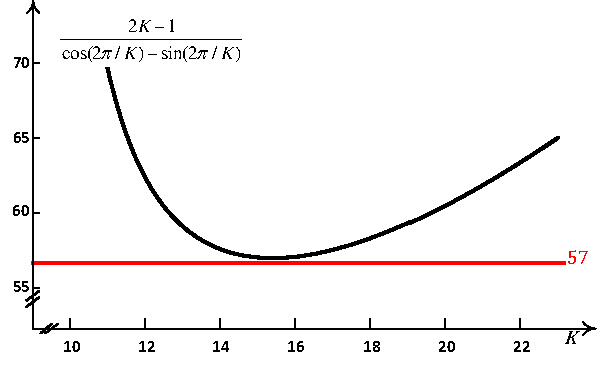
\includegraphics[scale=.7]{Figs/fig3.pdf}
  \vspace{-10pt}
  \caption{The function $\dfrac{2K-1}{\cos(2\pi/K)-\sin(2\pi/K)}$ }
  \label{fig:function}
\end{figure}


\section{The Proposed Algorithm for the Geometric FTP}
In this section, we introduce a constant factor approximation algorithm for the 2-dimensional geometric FTP, which runs in linear time. The main idea of our algorithm is to split the area, in which the robots are, and to solve the problem in a divide-and-conquer manner, by matching asleep robots to awake ones.\\
Assume there is one awake robot named $s$, and $R$ is the set of $n$ asleep robots (Note that in this section, $R$ does not include $s$); $d=diam(R)$ is the diameter of $R$, that is, the longest Euclidean distance between any two asleep robots; and $d_s$ is the radius of $R$ with respect to $s$, that is, the maximum Euclidean distance from $s$ to any member of $R$.\\
If so, an $a\times b-$rectangle with $a,b\leq d$, can be found, which encompasses positions of all members of $R$, while its sides are parallel to the axes. Let $A$ be such a rectangle (Figure~\ref{fig:split A}). \\
Our algorithm (let call it \textit{ApproxFTP} hereafter) inputs $s$ as the only awake robot, and $R$ as the set of the asleep robots, and provides an awaking schedule.\\
If $|R|\leq 3$, $s$ wakes up an (arbitrary) asleep robot. This is done in a time not longer than $d_s$. Then, there will be at most two asleep robots remaining, which can be woken up by the two awake robots working in parallel, in a time not more than $\sqrt{2}~d$. (Since the robots are in a rectangle whose length and width are at most $d$.) Therefore, the whole awakening process can be done within time $d_s+\sqrt{2}~d$.\\
For $|R|\geq 4$, the algorithm works recursively. First, we find the sets $R'$ and $R''$, by dividing $A$ and $R$ as described in the following:  (See Algorithm~\ref{alg:ApproxFTP} for the pseducode.)\\
Let $m(x_{m},y_{m})\in R$ be the (left) median of $R$ in the lexicographical order based on $x$ and then $y$ coordinates. (Which means, if the members of $R$ are sorted in order of their $x$ values, and members with equal $x$ value, are sorted in order of their $y$ values, $m$ will be the $\lceil\dfrac{n}{2}\rceil$th member.) A vertical line that passes through $m$, splits $A$ into two sub-rectangles. At least, one of these rectangles, say $A'$, has a horizontal side of length $a'\leq d/2$ (Figure~\ref{fig:split A}).\\
Denote by $R'$, the set of the robots of $R$ that are located in $A'$, including the robot $m$, if $n$ is even and $A'$ is the left sub-rectangle, and excluding $m$ otherwise. It is obvious that $R'$ has $\lfloor\dfrac{n}{2}\rfloor$ members.
\begin{figure} [h]
  \centering
  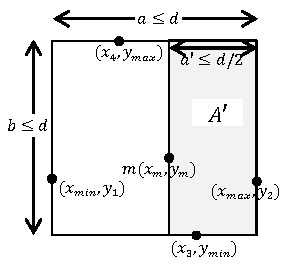
\includegraphics[scale=1]{Figs/fig4.pdf}
  \vspace{-15pt}
  \caption{Splitting the rectangle $A$ vertically.}
  \label{fig:split A}
\end{figure}\\
Now, let $m'(x_{m'},y_{m'})\in R'$ be the (left) median of $R'$ in the lexicographical order based on $y$ and then $x$ coordinates. Like the previous phase, a horizontal line that passes through $m'$ divides $A'$ into two rectangles, and at least one of them, say $A''$, has a vertical side of length $b''\leq d/2$. Note that the horizontal side of $A''$ is also of length $a''\leq d/2$ (Figure~\ref{fig:split A'}).\\
Denote by $R''$, the set of the robots of $R$ that are located in $A''$, including the robot $m'$ if $\lfloor\dfrac{n}{2}\rfloor$ is even and $A''$ is the bottom sub-rectangle, and excluding $m'$ otherwise. Obviously $R''$ has $\big\lfloor\dfrac{|R'|}{2}\big\rfloor \le \dfrac{n}{4}$ members.
\begin{figure} [h]
  \centering
  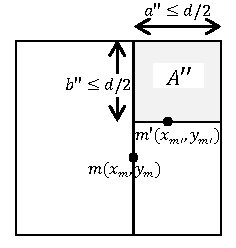
\includegraphics[scale=1]{Figs/fig5.pdf}
  \vspace{-15pt}
  \caption{Splitting the rectangle $A'$ horizontally.}
  \label{fig:split A'}
\end{figure}\\
Then, the algorithm runs with $s$ and $R''$ as inputs, to awake all the robots of $R''$. Notice that the awake robots are not necessarily in their initial places, but in (or very close to) places where some robots of $R''$ were initially there. Thus, all the awaken robots, including $s$, are located in $A''$.\\
Now, the number of the asleep robots remaining in $R'$, is less than or equal to the number of the awake robots, which are the members of $R''\cup\{s\}$:
$$ |R'-R''|=|R'|-\big\lfloor\dfrac{|R'|}{2}\big\rfloor \leq |R''|+1 $$
So, we assign to any robot of $R'-R''$, one of the robots of $R''\cup\{s\}$. To awake all the robots of $R'$, each of the asleep robots of $R'-R''$ can be awakened by its assigned robot of $R''\cup\{s\}$. Since the robots work in parallel, the time needed for this phase is bounded by the diagonal of $A'$, which is at most $\sqrt{5}/2~d$.\\
After this phase, $s$ and all the robots of $R'$ are awake, and all of them are located in $A'$. Here again, since the number of robots of $R-R'$ is not more than the number of the awake robots $R'\cup\{s\}$, they can be awaken in parallel in one phase. And the time needed to do this, is bounded by the diagonal of $A$, which is at most $\sqrt{2}~d$.
\begin{algorithm}
	\caption{ApproxFTP($R$, $s$)}
	\label{alg:ApproxFTP}
	\textbf{Input.} $R$: Set of asleep robots, $s$: An awake robot
	
	\algnewcommand{\lIf}[1]{\State\algorithmicif\ #1\ \algorithmicthen}
	\algnewcommand{\EndlIf}{\unskip\ \algorithmicend\ \algorithmicif}
	\begin{algorithmic}
		\If{$|R|\le3$}
		\State Assign $s$ to awake an (arbitrary) member $r$ of $R$.
		\State Assign $\{s,r\}$ to awake the members of $R-\{s\}$.
		\State \Return
		\Else \Comment $|R|\ge4$
		\State $m(x_m,y_m) \gets \big\lfloor\frac{|R|}{2}\big\rfloor$th member of $R$, in the lexicographical order based on $(x,y)$ coordinates
		\If {$(x_m-min\{x_r|r\in R\}) \le (max\{x_r|r\in R\}-x_m)$}
		\State $R'\gets\{~r \in R~|~x_r<x_m~or~(x_r=x_m~and~y_r<y_m)~\}$
		\lIf {$|R|$ is even} $R'\gets R'\cup\{m\}$ \EndlIf
		\Else \State $R'\gets\{~r \in R~|~x_r>x_m~or~(x_r=x_m~and~y_r>y_m)~\}$
		\EndIf
		
		\State $m'(x_{m'},y_{m'}) \gets \big\lfloor\frac{|R'|}{2}\big\rfloor$th member of $R'$, in the lexicographical order based on $(y,x)$ coordinates
		\If {$(y_{m'}-min\{y_r|r\in R'\}) \le (max\{y_r|r\in R'\}-y_{m'})$}
		\State $R''\gets\{~r \in R'~|~y_r<y_{m'}~or~(y_r=y_{m'}~and~x_r<x_{m'})~\}$
		\lIf {$|R'|$ is even} $R''\gets R''\cup\{m'\}$ \EndlIf
		\Else \State $R''\gets\{~r \in R'~|~y_r>y_{m'}~or~(y_r=y_{m'}~and~x_r>x_{m'})~\}$
		\EndIf
		
		\State ApproxFTP($R''$,$s$)
		\State Assign the members of $R''\cup\{s\}$ to awake the members of $R'-R''$.
		\State Assign the members of $R'\cup\{s\}$ to awake the members of $R-R'$.
		\EndIf
		\State \Return
	\end{algorithmic}
\end{algorithm}

\subsection{The Approximation Factor of ApproxFTP}
In this section, we assess the approximation factor of our proposed algorithm.

\begin{lemma}
\label{lem:1}
Suppose that $n$ asleep robots are located inside a rectangle, whose length and width are shorter than or equal to $d$, and there is an awake robot whose distance from the asleep robots is at most $d_s$. By applying \textit{ApproxFTP}, all asleep robots can be awaken within time ${ (2\sqrt{2}+\sqrt{5})d+d_s }$.
\end{lemma}
\begin{proof}
If $makespan(n,d)$ is the required time to wake up $n$ robots with the aforementioned conditions, for $n\geq4$ we have:
\begin{align}
makespan(n,d) &\leq makespan(\bigg\lfloor \dfrac{\lfloor\frac{n}{2}\rfloor}{2} \bigg\rfloor, \frac{d}{2})+\!\sqrt{2}d+\!\frac{\sqrt{5}}{2}d \nonumber\\
				&\leq makespan(\frac{n}{4}, \frac{d}{2})+(\sqrt{2}+\frac{\sqrt{5}}{2})d \nonumber
\end{align}
and for $n\le3$:
$$ makespan(n,d) \leq \sqrt{2} ~d+d_s $$
By solving this recurrence relation we have:
\begin{align}
makespan(n,d) &\leq (2\sqrt{2}+\!\sqrt{5})d-\!(\sqrt{2}+\!\frac{\sqrt{5}}{2}) 2^{-\!\lfloor\log_4n \rfloor}+d_s \nonumber\\
				&\leq (2\sqrt{2}+\!\sqrt{5})d+d_s \nonumber
\end{align}
\end{proof}
It is worth mentioning, that in the first call of the algorithm, in which $d=diam(R)$, the distance between each pair of robots is less than or equal to $d$, while in the next calls, the distance of two robots can be as long as the diagonal of the encompassing rectangle. This is the same distance that has appeared as $\sqrt{5}/2~d$ and $\sqrt{2}~d$ in our computations. But only for the first call, we can be assured that the distance of the robots is at most $d$, instead of $\sqrt{5}/2~d$ and $\sqrt{2}~d$. The following lemma uses this.

\begin{lemma}
\label{lem:2}
By applying \textit{ApproxFTP} algorithm, the required time for awaking $n$ asleep robots, whose positions are given by a set $R$, using one awake robot, whose distance from the asleep robots is at most $d_s$, is shorter than or equal to ${ (2+\sqrt{2}+\sqrt{5}/2)diam(R)+d_s }$.
\end{lemma}
\begin{proof}
In the first call of the algorithm, the distance of the robots from each other is at most $diam(R)$. So, after awaking all the robots of $R''$, the other robots of $R$ can be woken up in two phases, each of a time not more than $diam(R)$. Hence:
$$ makespan(R) \leq makespan(\frac{n}{4},\frac{diam(R)}{2})+2diam(R) $$
For next call of the algorithm, we use Lemma~\ref{lem:1}:
$$ makespan(\frac{n}{4},\frac{diam(R)}{2}) \leq (2\sqrt{2}+\!\sqrt{5})\frac{diam(R)}{2}+d_s $$
and as a result:
\begin{align}
makespan(R) &\leq (2\sqrt{2}+\!\sqrt{5})\frac{diam(R)}{2}+d_s+2~diam(R) \nonumber\\
			&\leq (2+\sqrt{2}+\frac{\sqrt{5}}{2})diam(R)+d_s \nonumber
\end{align}
\end{proof}

\begin{theorem}
\textit{ApproxFTP} is an approximation algorithm, with a constant approximation factor less than $10.1$.
\end{theorem}
\begin{proof}
In the previous lemma, it was proven that:
$$ makespan(R) \leq (2+\sqrt{2}+\frac{\sqrt{5}}{2})diam(R)+d_s $$
We know that $diam(R)\leq2d_s$, because, if we draw a circle with $s$ as the center, and $d_s$ as the radius, it will encompass all of the robots of $R$. Hence:
$$ makespan(R) \leq (5+2\sqrt{2}+\sqrt{5})d_s < 10.1~d_s $$
Since $d_s$ is a lower bound for the optimum makespan, the approximation factor of \textit{ApproxFTP} that is less than $10.1$.
\end{proof}

\subsection{The Time Complexity of ApproxFTP}
To compute the time complexity of this algorithm, it should be noted, that finding the median of a set with $n$ members, can be done in $O(n)$ time~\cite{CLRS}. So, the algorithm can find $A'$, $A''$, $R'$ and $R''$ in $O(n)$ time. Then, the algorithm is called with $R''$ as its input. The number of the members of $R''$ is less than or equal to $n/4$. After that, the algorithm finds matchings between the members of $R'-R''$ and $R''\cup\{s\}$, and the members of $R-R'$ and $R'\cup\{s\}$. This phases can also be done in $O(n)$.\\
So, if the running time of algorithm for $|R|=n$ is shown as $T(n)$,
\begin{align}
T(n)&=T(\frac{n}{4})+O(n) &n\geq 4 \nonumber\\
T(n)&=O(1) &n\leq 3 \nonumber
\end{align}
By solving this recursive relation, we find out that $T(n)=O(n)$.


\section{Conclusion}
In this paper, we considered the Freeze-Tag Problem, which is NP-Hard in general, and its geometric variant is an open problem. Then, a constant factor linear-time approximation algorithm for the 2-dimensional geometric Freeze-Tag Problem was introduced.

\section*{References}

\bibliography{FTPbib}

\end{document}